 \chapter{Anyagi pont rezg\'esei}
 
 \section{Mechanika} 
  
  \subsection{Rezgések általában}
   
   A csillapított gerjesztett rezgések mozgásegyenlete:
   \al{
    m\ddot x=-Dx-k\dot x +F(t),
   }
   ahol $D$ a direkciós állandó, $k$ a csillapítás, $m$ a tömeg és $F(t)$ a gerjesztő erő. $m$-mel elosztva és bevezetve új jelöléseket:
   \al{
    &\beta=\frac{k}{2m}
    &\omega_0^2=\frac{D}{m}
    &&f(t)=\frac{F(t)}{m},
   }
   \al{
    \ddot x+2\beta\dot x+\omega_0^2 x=f(t).
   }
   \paragraph{Homogén egyenlet megoldása}
    
    A homogén egyenlet ($f(t)\equiv 0$) megoldásait keressük $x(t)=Ae^{\lambda t}$ alakban. Behelyettesítve:
    \al{
     0&=\ddot x+2\beta\dot x+\omega_0^2 x
       =\lambda^2 A e^{\lambda t}+2\beta\lambda Ae^{\lambda t}+\omega_0^2 Ae^{\lambda t}
       =\big(\lambda^2  +2\beta\lambda +\omega_0^2 \big)e^{\lambda t},
    }
    ami akkor teljesül, ha 
    \al{
     \lambda_{12}
      =\frac{-2\beta\pm\sqrt{4\beta^2-4\cdot\omega_0^2}}{2}
      =-\beta\pm\sqrt{\beta^2-\omega_0^2}.
    }
    
    \begin{itemize}
     \item {\bf Erősen csillapított eset: $\beta>\omega_0$}
     
     Ekkor a két valós $\lambda$ értéke különbözik, így az általános megoldás:
     \al{
      x(t)
       &=A_1 e^{\big(-\beta+\sqrt{\beta^2-\omega_0^2}\big)t}+A_2 e^{\big(-\beta-\sqrt{\beta^2-\omega_0^2}\big)t}\\
%        &=\tilde{A}_1 e^{-\beta t}\left(e^{\sqrt{\beta^2-\omega_0^2 }t}+\tilde{A}_2e^{-\sqrt{\beta^2-\omega_0^2 }t}\right).
     }
     
     Ennek illesztése a kezdeti feltételekhez: legyen $t_0$-ban a test $x=0$-ban és legyen $v_0$ sebessége. Ekkor a megoldás:
     \al{
      &\left.
      \begin{array}{r}
       A_1+A_2=0\\
       \lambda_1A_1+\lambda_2A_2=v_0
      \end{array}
      \right\}
      &\Rightarrow
      &&\begin{array}{l}
         A_1=-\frac{v_0}{\lambda_2-\lambda_1}=\frac{v_0}{2\sqrt{\beta^2-\omega_0^2}}\\
         A_2=\frac{v_0}{\lambda_2-\lambda_1}=-\frac{v_0}{2\sqrt{\beta^2-\omega_0^2}}
        \end{array}
     }
     \al{
      x(t)
       &=\frac{v_0}{2\sqrt{\beta^2-\omega_0^2}}e^{-\beta t}\left(e^{\sqrt{\beta^2-\omega_0^2}t}-e^{-\sqrt{\beta^2-\omega_0^2}t}\right)
        =\frac{v_0}{\sqrt{\beta^2-\omega_0^2}}e^{-\beta t}\sh\left(\sqrt{\beta^2-\omega_0^2}t\right).
     }
     \item {\bf Határeset: $\beta=\omega_0$}
      
      Ekkor csak egy $\lambda$ érték van. Az egyenlet másodrendű, így kell lennie egy másik független megoldásnak. Ezt keressük a $x(t)=Ate^{\lambda t}$ alakban:
      \al{
       0&=\ddot x+2\beta\dot x+\omega_0^2 x
        =A\left(2\lambda e^{\lambda t}+\lambda^2 t e^{\lambda t}\right)+A2\beta\left(e^{\lambda t}+\lambda t e^{\lambda t}\right)+\beta^2 A t e^{\lambda t}\\
       &=e^{\lambda t}
       \Big(2(\lambda +\beta)+(2\beta\lambda +\lambda^2+\beta^2 )t\Big),
      }
      ami akkor teljesül, ha $\lambda=-\beta$. Így
      \al{
       x(t)=Ae^{-\beta t}+B t e^{-\beta t}.
      }
      A kezdeti feltételekhez hasonlóan illeszthető.
      
     \item {\bf Gyengén csillapított eset: $\beta<\omega_0$}
      
      Ekkor a két megoldás szintén független, a gyökök alatt negatív szám áll. Ezzel a megoldások:
      \al{
       &\sqrt{\beta^2-\omega_0^2}=i\sqrt{\omega_0^2-\beta^2}=i\omega
       &x(t)=A_1 e^{-\beta t-i\omega t}+A_2 e^{-\beta t+i\omega t}.
      }
      A megoldás akkor lesz valós, ha $A_2=A_1^*$. Vezessük be az $A_1=\frac{1}{2}Ae^{i\delta}$ jelölést, ahol $A$ valós, így
      \al{
       x(t)
        &=A\frac{1}{2}\left(e^{-\beta t-i\omega t+i\delta}+e^{-\beta t+i\omega t-i\delta}\right)
         =Ae^{-\beta t}\frac{1}{2}\left(e^{-i\omega t+i\delta}+e^{+i\omega t-i\delta}\right)\\
        &=Ae^{-\beta t}\cos\left(\omega t-\delta\right),
      } 
      ami egy harmonikus rezgés $\omega$ frekvenciával, melynek amplitúdója lecseng. 
    \end{itemize}
    
   \paragraph{Az inhomogén egyenlet megoldása}
    
    Legyen a gerjesztés speciális $f(t)=f_0\cos(\Omega t)=\Re\big[e^{i\Omega t} \big]$. Keressünk egy partikuláris megoldást, melynek frekvenciája megfelel a gerjesztésnek:
    \al{
     x_p(t)=\Re\big[Ae^{i\Omega t}\big],
    }
    melyet behelyettesítve:
    \al{
     f_0 e^{i\Omega t}
      &=-\Omega^2 Ae^{i\Omega t}+2i\beta\Omega Ae^{i\Omega t}+\omega_0^2 Ae^{i\Omega t}\\
     f_0 
      &=-\Omega^2 A+2i\beta\Omega A+\omega_0^2 A\\
     A&=\frac{f_0}{\omega_0^2-\Omega^2 +2i\beta\Omega},
    }
    ahonnan:
    \al{
     &A=\abs{A}e^{i\delta}
     &\abs{A}=\frac{f_0}{\sqrt{\big(\omega_0^2-\Omega^2)^2 +4\beta^2\Omega^2}}
     &&\delta=\arctan\left(\frac{-2\beta\Omega}{\omega_0^2-\Omega^2}\right),
    }
    így
    \al{
     x_p(t)
      =\Re\big[Ae^{i\Omega t}\big]
      =\abs{A}\cos(\Omega t + \delta)
      =\frac{f_0}{\sqrt{\big(\omega_0^2-\Omega^2)^2 +4\beta^2\Omega^2}}\cos(\Omega t + \delta).
    }
    
    A teljes megoldás tehát a homogén megoldások és a partikuláris megoldások összege, de láttuk, hogy a homogén megoldások exponenciálisan lecsengenek a csillapítással, így hosszú idő múlva már csak a partikuláris megoldás marad. 
    
  \subsection{Rezgések Lagrange- és Hamilton-formalizmusa}
   
   A szabad harmonikus rezgőmozgás egyenleteit lásd \aref{ss:11-kanonikusperturbacioszamitas}. fejezetben. 
   
   A csillapított rezgés Lagrange-függvénye:
   \al{
    L=e^{\frac{k}{m}t}\left[\frac{1}{2}m\dtx^2 -\frac{1}{2}D x^2 \right].
   }
   A mozgásegyenlet ebből:
   \al{
    0&=\der{}{t}\pder{L}{\dtx}-\pder{L}{x}
      =\der{}{t}\left(e^{\frac{k}{m}t}m\dtx\right)+e^{\frac{k}{m}t}D x
      =e^{\frac{k}{m}t}\left(\frac{k}{m}m\dtx+m\ddtx+D x\right)\\
     &=e^{\frac{k}{m}t}\left(m\ddtx+k\dtx+D x\right).
   }
   
   A Hamilton-függvény:
   \al{
    H&=p\dtx-L
      =\pder{L}{\dtx}\dtx-L
      =\left(e^{\frac{k}{m}t}m\dtx\right)\dtx-e^{\frac{k}{m}t}\left[\frac{1}{2}m\dtx^2 -\frac{1}{2}D x^2 \right]
      =e^{\frac{k}{m}t}\left[\frac{1}{2}m\dtx^2 +\frac{1}{2}D x^2 \right]\\
     &=\frac{1}{2m} p^2 e^{-\frac{k}{m}t} +\frac{1}{2}D x^2 e^{\frac{k}{m}t}.\\
   }
   A kanonikus egyenletek:
   \al{
    \dtx&=\pder{H}{p}=\frac{1}{m} p e^{-\frac{k}{m}t} &\Rightarrow && p=m\dtx e^{\frac{k}{m}t}\\
    \dtp&=-\pder{H}{x}=-D x e^{\frac{k}{m}t}.
   }
   Az első egyenletbe idő szerint deriválva, majd a másodikat behelyettesítve:
   \al{
    \big(m\ddtx +k\dtx \big)e^{\frac{k}{m}t}
     =\dtp
     =-D x e^{\frac{k}{m}t},
   }
   vagyis 
   \al{
    0=\big(m\ddtx +k\dtx +D x\big)e^{\frac{k}{m}t},
   }
   ami visszaadja a helyes mozgásegyenletet. Ennek a megoldása kis csillapításra láttuk, hogy 
   \al{
    x(t)=e^{-\frac{k}{2m}t}\Big(A_1\cos(\omega t)+A_1\sin(\omega t)\Big),
   }
   a konjugált impulzus:
   \al{
    \dtp(t)
     =-D x e^{\frac{k}{m}t}
      \sim e^{\frac{k}{2m}t},
   }
   így az végtelenhez fog tartani, ahogy az idő telik. Ez van, nem probléma, mert a valóságban nem a kanonikus impulzust mérjük, hanem a kinetikusat, az pedig $k=m\dtx\sim e^{-\frac{k}{m}t}$-vel lecseng, ahogy várjuk.
   
  \subsection{Kanonikus transzformációk}
   
   \paragraph{Transzformáció egyenes vonalú egyenletes mozgássá}
    
    Tekintsünk egy harmonikus oszcillátort, amelyben nincs csillapítás. Ekkor 
    \al{
     H=\frac{1}{2m}p^2+\frac{1}{2}Dx^2.
    }
    Végezzünk el egy 1.\ típusú kanonikus transzformációt:
    \aln{
     &W_1(x,X,t)=\frac{\sqrt{mD}}{2}x^2\ctg X
     &p=\pder{W_1}{x}
     &&P=-\pder{W_1}{X}
     &&H'=H+\pder{W_1}{t}.
    }
    Innen
    \al{
     &p=\sqrt{mD}x\ctg X
     &P=\frac{\sqrt{mD}}{2}x^2\frac{1}{\sin^2 X}
    }
    \al{
     H'(X,P)
     &=H(x,p)
      =\frac{1}{2m}\left(\sqrt{mD}x\ctg X\right)^2+\frac{1}{2}D\left(\frac{2\sin^2 X}{P\sqrt{mD}}\right)\\
     &=\frac{1}{2m}mD \left(\frac{2P\sin^2 X}{\sqrt{mD}}\right)\ctg^2 X+\frac{1}{2}D\left(\frac{2P\sin^2 X}{\sqrt{mD}}\right)\\
     &=\sqrt{\frac{D}{m}}P\cos^2 X+\sqrt{\frac{D}{m}}P\sin^2 X
      =\sqrt{\frac{D}{m}}P
      =\omega P.
    }
    A kanonikus egyenletek:
    \al{
     \dot{X}&=\omega &\Rightarrow &&X(t)=\omega t+ X_0,&&
     \dot{P}&=0 &\Rightarrow &&P(t)=P_0.
    }
    Az eredeti koordinátákban:
    \al{
     x=\sqrt{\frac{2P}{\sqrt{mD}}}\sin X=\sqrt{\frac{2P_0}{\sqrt{mD}}}\sin (\omega t + X_0).
    }
    
   \paragraph{Csillapított rezgést csillapítatlanba}
    
    Tekintsünk egy csillapított rezgést:
    \al{
     H=\frac{1}{2m} p^2 e^{-\frac{k}{m}t} +\frac{1}{2}D x^2 e^{\frac{k}{m}t}.
    }
    Itt is egy 1-es típusú kanonikus transzformációt fogunk alkalmazni:
    \al{
     W_1(x,X,t)
      &=-xXe^{\frac{k}{2m}t}-\frac{k}{4}x^2 e^{\frac{k}{m}t}\\
     p
      &=\pder{W_1}{x}
       =-Xe^{\frac{k}{2m}t}-\frac{k}{2}x e^{\frac{k}{m}t}
      &\Rightarrow
      &&p&=-\left(X+\frac{k}{2}P\right)e^{\frac{k}{2m}t}\\
     P
      &=-\pder{W_1}{X}
       =xe^{\frac{k}{2m}t}
      &\Rightarrow
      &&x&=Pe^{-\frac{k}{2m}t}
    }
    \al{
    H'
      &=H+\pder{W_1}{t}
       =\frac{1}{2m} p^2 e^{-\frac{k}{m}t} +\frac{1}{2}D x^2 e^{\frac{k}{m}t}-xX\frac{k}{2m}e^{\frac{k}{2m}t}-\frac{k}{4} \frac{k}{m} x^2e^{\frac{k}{m}t}\\
      &=\frac{1}{2m} \left(\left(X+\frac{k}{2}P\right)e^{\frac{k}{2m}t}\right)^2 e^{-\frac{k}{m}t}
        +\frac{1}{2}D \left(Pe^{-\frac{k}{2m}t}\right)^2 e^{\frac{k}{m}t}
        -\left(Pe^{-\frac{k}{2m}t}\right)X\frac{k}{2m}e^{\frac{k}{2m}t}\\
      &\qquad-\frac{k}{4} \frac{k}{m} \left(Pe^{-\frac{k}{2m}t}\right)^2 e^{\frac{k}{m}t}\\
      &=\frac{1}{2m} \left(X^2+kPX+\frac{k^2}{4}P^2\right)
        +\frac{1}{2}D P^2
        -PX\frac{k}{2m}
        -\frac{k}{4} \frac{k}{m} P^2 \\
      &=\frac{1}{2m}X^2+\frac{1}{2}m\underbrace{\left(\frac{D}{m}-\frac{k^2}{4m^2}\right)}_{=\Omega^2}P^2.
    }
    Ez egy harmonikus oszcillátor. Azért a kanonikus egyenletek:
    \al{
     &\dot{P}=-\pder{H'}{X}=\frac{1}{m}X
     &\dot{X}=\pder{H'}{P}=m\Omega^2 P,
    }
    ahonnan
    \al{
     &\ddot{X}+\Omega^2 X=0
     &\Rightarrow
     &&\left\{
       \begin{array}{l}
        X(t)=A\sin(\Omega t+\varphi)\\
        P(t)=A\cos(\Omega t+\varphi).
       \end{array}
       \right.,
    }
    vagyis 
    \al{
     x(t)&=P(t) e^{-\frac{k}{2m}t}=Ae^{-\frac{k}{2m}t}\cos(\Omega t+\varphi)\\
     p(t)&=-\left(X(t)+\frac{k}{2}P(t)\right)e^{\frac{k}{2m}t}
       =-\left(A\sin(\Omega t+\varphi)+\frac{k}{2}A\cos(\Omega t+\varphi)\right)e^{\frac{k}{2m}t}\\
      &=B\sin(\Omega t+\vartheta)e^{\frac{k}{2m}t}.
    }
    Örömteli módon ez a megoldás is megegyezik a korábbiakkal.
    
   \paragraph{Komplex kanonikus transzformáció (Wow!!!)}
    
    Az ideális harmonikus rezgéshez keresünk új koordinátákat:
    \al{
     H=\frac{1}{2m}p^2+\frac{1}{2}Dx^2.
    }
    Mátrixos alakban a transzformáció: 
    \al{
     &\begin{pmatrix}
      X\\P
     \end{pmatrix}
     =\frac{1}{\sqrt{2m\omega}}
     \begin{pmatrix}
      m\omega & i\\
      im\omega & 1
     \end{pmatrix}
     \begin{pmatrix}
      x\\p
     \end{pmatrix}
     &\begin{array}{l}
       \displaystyle x=\sqrt{\frac{1}{2m\omega}}\big(X-iP\big)\\
       \displaystyle p=\sqrt{\frac{m\omega}{2}}\frac{1}{i}\big(X+iP\big)
      \end{array}
    }
    Ez kanonikus transzformáció, mert $\{X,P\}=\pder{P}{p}\pder{X}{x}-\pder{P}{x}\pder{X}{p}=1=\{x,p\}$. $\omega$ eddig még csak egy valós szám, később rögzítjük. A Hamilton:
    \al{
     H'
      &=\frac{1}{2m}\left(\sqrt{\frac{m\omega}{2}}\frac{1}{i}\big(X+iP\big)\right)^2+\frac{1}{2}D\left(\sqrt{\frac{1}{2m\omega}}\big(X-iP\big)\right)^2\\
      &=-\frac{1}{2m}\frac{m\omega}{2}\big(X+iP\big)^2+\frac{1}{2}D\frac{1}{2m\omega}\big(X-iP\big)^2\\
      &=-\frac{\omega}{4}\big(X^2+2iXP-P^2\big)+\frac{D}{4m\omega}\big(X^2-2iXP-P^2\big)\\
      &=-\frac{\omega}{4}\big(X^2+2iXP-P^2\big)+\frac{D}{4m\omega}\big(X^2-2iXP-P^2\big)
    }
    Itt már látjuk, hogy $\omega^2=\frac{D}{m}$ kifizetődő választás, ugyanis:
    \al{
     H'
      &=-\frac{\omega}{4}\big(X^2+2iXP-P^2\big)+\frac{\omega}{4}\big(X^2-2iXP-P^2\big)
       =-i\omega XP.
    } 
    A kanonikus egyenletek:
    \al{
     &\dot{P}=-\pder{H'}{X}=i\omega P
     &\Rightarrow
     &&P(t)&=P_0e^{i\omega t}\\
     &\dot{X}=\pder{H'}{P}=-i\omega X
     &\Rightarrow
     &&X(t)&=X_0 e^{-i\omega t}
    }
    Az új Lagrange: $H'=P\dot{X}-L'$ $\Rightarrow$ $L'=P\dot{X}-H'=-i\omega XP+i\omega XP=0$.
    
    Bizony. A kanonikus transzformációk kivezetnek azon Lagrange-függvények halmazából, amelyekhez tartozik fizikai rendszer. 
    
 
 \section{Elektrodinamika}
  
  \subsection{Dipólsugárzás}
   
   Az oszcilláló töltésrendszerek sugárzásához lásd \aref{ss:13-oszcillaloter}. fejezetet.
   
   A vektorpotenciál sorfejtett alakja (\eqref{eq:13-vectpot} egyenlet):
   \al{
    \vect{A}(\omega,\rv)
      &=\frac{\mu_0}{4\pi}\frac{e^{ikr}}{r}\intl{}{}\dd^3\rv'\,\vect{J}(\rv')\big(1-ik\rv'\ev_\rv\big).
   }
   
   Csak az első tagot tartjuk meg az előzőben, és az integrált átalakítjuk:
   \al{
    \intl{}{}\dd^3\rv'\,\vect{J}_i(\rv)
     &=\intl{}{}\dd^3\rv'\,\vect{J}_j(\rv)\partial_j r_i
      =-\intl{}{}\dd^3\rv'\,\partial_j\vect{J}_j(\rv) r_i
      =\intl{}{}\dd^3\rv'\,\partial_t\rho(\rv) r_i
      =\partial_t\intl{}{}\dd^3\rv'\,\rho(\rv) r_i\\
     &=\partial_t p_i
      =-i\omega p_i,
   }
   ahol $\pv$ a dipólmomentum. Ezzel
   \al{
    \vect{A}(\omega,\rv)
     &=-i\omega\frac{\mu_0}{4\pi}\frac{e^{ikr}}{r}\pv.
   }
   
   A terek előállításakor is csak az $\frac{1}{r}$-rel arányos tagokat tartjuk meg:
   \al{
    \partial_j\frac{e^{ikr}}{r}
     &=\frac{1}{r}\partial_j e^{ikr}+\mathcal{O}\left(\frac{1}{r^2}\right)
     =\frac{1}{r}ik r_j\frac{1}{r}e^{ikr}+\mathcal{O}\left(\frac{1}{r^2}\right),
     &\vects{\nabla}\to ik \ev_\rv
   }
   így:
   \al{
    \Hv
     &=\frac{1}{\mu_0}\rot{\Av}
      =-\frac{1}{\mu_0}i\omega\frac{\mu_0}{4\pi}\frac{e^{ikr}}{r}ik\ev_\rv\times\pv
      =\frac{k\omega}{4\pi}\frac{e^{ikr}}{r}\ev_\rv\times\pv
      =\frac{\omega^2}{4\pi c}\frac{e^{ikr}}{r}\ev_\rv\times\pv,\\
    \Ev
     &=\frac{ic^2}{\omega}\rot{\Bv}
      =\frac{ic^2}{\omega}ik\ev_\rv\times\Bv
      =c\Bv\times\ev_\rv
      =\mu_0 c\Hv\times\ev_\rv
      =Z_0\Hv\times\ev_\rv,
   }
   ahol $Z_0=376.7\,\Omega$ a vákuumimpedancia. A Poynting-vektor:
   \al{
    \Sv
     =\Ev\times\Hv
     =Z_0\big(\Hv\times\ev_\rv\big)\times\Hv
     =Z_0\Hv^2\ev_\rv,
   }
   melyet egy teljes periódusra átlagolva $e^{i2kr}\to 1/2$:
   \al{
    \mv{\Sv}_t
     =\frac{1}{2}Z_0\mv{\Hv^2}_t
     =\frac{1}{2}Z_0\frac{\omega^4}{16\pi^2 c^2}\frac{1}{r^2}\pv^2\sin^2\vartheta,
   }
   ahol $\pv$ és $\rv$ között a bezárt szög $\vartheta$. A legegyszerűbb, ha $z$ irányba mutat a dipól, és $\rv$ pedig a gömbi koordináta-rendszerben a helyvektor. $\Sv$ integrálva egy zárt felületre a dipól által kisugárzott teljesítményt adja (a gömbön $\ev_\rv$ merőleges a felületre, így):
   \aln{
    \dd P&=\dd\Omega r^2 \me{\Sv}_t\ev_\rv
    \qquad\qquad\qquad\der{P}{\Omega}=Z_0\frac{\omega^4}{32\pi^2 c^2}\pv^2\sin^2\vartheta\nonumber\\
    P&
      =\intl{}{}\dd\Omega Z_0\frac{\omega^4}{32\pi^2 c^2}\pv^2\sin^2\vartheta
      =Z_0\frac{\omega^4}{32\pi^2 c^2}\pv^2 2\pi\intl{-1}{1}\dd(\cos\vartheta) \sin^2\vartheta
      =Z_0\frac{\omega^4}{32\pi^2 c^2}\pv^2 2\pi\frac{4}{3}\\
     &=Z_0\frac{\omega^4}{12\pi c^2}\pv^2\label{eq:13-dipolsug}
   }
   
  \subsection{Hertz-vektor}
   
   Lorentz-mértékben $\left(\divo \Av+\frac{1}{c^2}\partial_t\phi=0\right)$ a potenciálokat d'Alambert-egyen\-letek határozzák meg:
   \al{
     &\left(\Delta-\frac{1}{c^2}\partial_t^2\right)\phi=-\frac{1}{\ep_0}\rho  &\left(\Delta-\frac{1}{c^2}\partial_t^2\right)\vect{A}=-\mu_0\vect{J}. 
    }
   
   A vektorpotenciál három komponense és a skalárpotenciál összesen négy darab háromváltozós függvény. Ez a leírás kicsit redundáns a mértékinvariancia miatt. Mértéket választva ezek már nem független egymástól, így érdemes áttérni egy olyan leírásra, ahol csak három függvénnyel kell foglalkozni.
   
   Vezessünk be új potenciálokat. Legyen $\Piv(t,\rv)$ olyan, hogy 
   \al{
    &\Av=\frac{1}{c^2}\partial_t\Piv.\\
    &\frac{1}{c^2}\partial_t\phi=-\divo\Av=-\frac{1}{c^2}\partial_t\divo\Piv
    &\Rightarrow
    &&\phi=-\divo\Piv.
   }
   Ha nincsenek források, vagy $\rho=0$ és $\Jv=0$, akkor a $\phi$-re vonatkozó egyenletbe behelyettesítve:
   \al{
    &\divo\left[\left(\Delta-\frac{1}{c^2}\partial_t^2\right)\Piv\right]=0
    &\Rightarrow
    &&\left(\Delta-\frac{1}{c^2}\partial_t^2\right)\Piv=0.
   }
   
   Az új potenciállal kifejezve a terek:
   \al{
    &\Bv=\rot\Av
     =\frac{1}{c^2}\partial_t\rot\Piv
    &\Hv=\ep_0\partial_t\rot\Piv
   }
   \al{
    \Ev
     &=-\partial_t\Av-\grad\phi
      =-\frac{1}{c^2}\partial_t^2\Piv+\grad(\divo\Piv)
      =-\frac{1}{c^2}\partial_t^2\Piv+\rot(\rot\Piv)+\Delta\Piv\\
     &=\left(\Delta-\frac{1}{c^2}\partial_t^2\right)\Piv+\rot(\rot\Piv)
      =\rot(\rot\Piv)
   }
  
 \section{Kvantummechanika}
  
  \subsection{Harmonikus oszcillátor}
   
   A Hamilton-operátor koordináta-reprezentációban:
   \al{
    \opH=\frac{1}{2m}\opp^2+\frac{1}{2}m\omega^2\opx^2
     =-\frac{\hbar^2}{2m}\Delta+\frac{1}{2}m\omega^2 x^2,
   }
   így a Schrödinger-egyenlet:
   \al{
    \left(-\frac{\hbar^2}{2m}\Delta+\frac{1}{2}m\omega^2 x^2\right)\psi(x)=E\psi(x).
   }
   
   Először tegyük dimenziótlanná az egyenletet:
    \al{
     &\xi=\frac{x}{x_0}
     &x_0=\sqrt{\frac{\hbar}{m\omega}}
     &&\eta=\frac{2E}{\hbar\omega},
    }
    melyekkel:
    \aln{
     \left(\Delta_\xi+\eta-\xi^2\right)\psi(\xi)=0.\label{eq:16-nodimenz}
    }
    
   \paragraph{Megoldás Sommerfeld-féle polinom módszerrel}
    
    Az aszimptotikus megoldás $\xi\to\pm\infty$-re: ekkor $\eta$ elhagyható $q^2$ mellett. Az egyenletnek megoldása $\psi_\text{a}(\xi)=e^{-\frac{\xi^2}{2}}$. Behelyettesítve:
    \al{
     \left(\Delta_\xi-\xi^2\right)\psi_\text{a}(\xi)
      &=\left(\Delta_\xi-\xi^2\right)e^{-\frac{\xi^2}{2}}
       =-e^{-\frac{\xi^2}{2}}+\xi^2 e^{-\frac{\xi^2}{2}}
        -\xi^2 e^{-\frac{\xi^2}{2}}
       =-e^{-\frac{\xi^2}{2}}\xrightarrow{\xi\to\pm\infty}=0.
    }
    A teljes megoldást keressük egy másik függvény és az aszimptotikus alak szorzataként:
    \al{
     \psi(\xi)=u(\xi)\psi_\text{a}(\xi). 
    }
    Ekkor az $u(\xi)$-re kapott differenciálegyenlet:
    \al{
     0&=\left(\Delta_\xi+\eta-\xi^2\right)\psi(\xi)
       =\left(\Delta_\xi+\eta-\xi^2\right)u(\xi)\psi_\text{a}(\xi)\\
      &= u''(\xi)\psi_\text{a}(\xi)-u'(\xi)\xi\psi_\text{a}(\xi) -u'(\xi)\xi\psi_\text{a}(\xi)-u(\xi)\psi_\text{a}(\xi) +u(\xi)\xi^2\psi_\text{a}(\xi)\\
      &\qquad+\eta u(\xi)\psi_\text{a}(\xi)-\xi^2 u(\xi)\psi_\text{a}(\xi)\\
      &=\psi_\text{a}(\xi)\big( u''(\xi)-2u'(\xi)\xi+u(\xi)\xi^2
       +(\eta-1) u(\xi)-\xi^2 u(\xi)\big)\\
      &=\psi_\text{a}(\xi)\big( u''(\xi)-2u'(\xi)\xi+(\eta -1) u(\xi)\big)\\
      0&=u''(\xi)-2u'(\xi)\xi+(\eta-1) u(\xi)
    }
    Keressük az $u(\xi)$ függvényt hatványsor alakban:
    \al{
     u(\xi)&=\suml{i=0}{\infty}c_i\xi^i\\
     u'(\xi)&=\suml{i=0}{\infty}ic_i\xi^{i-1}\\
     u''(\xi)&=\suml{i=2}{\infty}i(i-1)c_i\xi^{i-2}
              = \suml{i=0}{\infty}(i+1)(i+2)c_{i+2}\xi^{i}.
    }
    Behelyettesítve a differenciálegyenletbe:
    \al{
     0&=\suml{i=0}{\infty}(i+1)(i+2)c_{i+2}\xi^{i}-2\xi\suml{i=0}{\infty}ic_i\xi^{i-1}+(\eta-1) \suml{i=0}{\infty}c_i\xi^{i}\\
      &=\suml{i=0}{\infty}\Big[(i+1)(i+2)c_{i+2}-2ic_i+(\eta-1)c_i\Big]\xi^{i}.
    }
    Az együtthatóknak minden $i$ indexre el kell tűnni, így
    \al{
     c_{i+2}=\frac{2i-\eta+1}{(i+1)(i+2)}c_i.
    }
    Láthatjuk, hogy csak minden második index van összekötve, így a $c_0=1$ $c_1=0$ és a $c_0=0$ $c_1=1$ választással a másodrendű differenciálegyenlet két független megoldását elő lehet állítani. Az első esetben páros, a másodikban pedig páratlan függvényt kapunk. 
    
    Aszimptotikusan a rekurziós összefüggés közelíthető $c_{i+2}\sim\frac{2}{1}c_i$, vagyis aszimptotikusan $u(\xi)\to e^{\xi^2}$. Hiszen $e^{\xi^2}=\suml{i=0}{\infty}\frac{\xi^{2i}}{i!}=\suml{\substack{i=0\\ (k=2i)}}{\infty}\frac{\xi^{k}}{(k/2)!}$, vagyis $c_i=\frac{1}{(i/2)!}$, így $\frac{c_{i+2}}{c_i}=\frac{1}{i/2+1}=\frac{2}{i+2}\xrightarrow{i\to\infty}\frac{2}{i}$.
    
    De ha $u(\xi)\sim e^{\xi^2}$ aszimptotikusan, akkor a megoldás $\psi(\xi)\sim e^{\frac{\xi^2}{2}}$, ami viszont nem normálható. Normálható megoldást akkor kapunk, ha létezik olyan $n$, hogy $c_{n+2}=0$, vagyis
    \al{
     &0=2n+1-\eta=2n+1-\frac{2E_n}{\hbar\omega}
     &\Rightarrow
     &&E_n=\hbar\omega \left(n+\frac{1}{2}\right)\qquad n=0,1,2,\dots
    }
    
    A sajátfüggvények 
    \al{
     \psi_n(x)=\frac{1}{\sqrt{2^n n!\sqrt{\pi} \, x_0}}H_n\left(\frac{x}{x_0}\right)e^{-\frac{x^2}{2 x_0^2}},
    }
    ahol a Hermite-polinomok:
    \al{
     &H_n(\xi)=(-1)^n e^{\xi^2}\frac{\dd^n}{\dd \xi^n}e^{-\xi^2}
     &\intl{-\infty}{\infty} H_m(\xi) H_n(\xi)\, e^{-\xi^2}\, \dd \xi = 2^n n! \sqrt{ \pi}  \delta_{nm}
    }
    \begin{figure}[ht!]
     \centering
     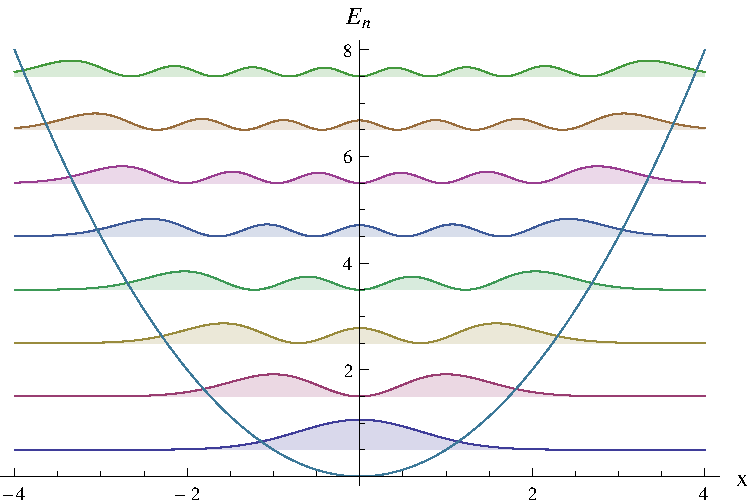
\includegraphics[width=0.7\textwidth]{A16tetel/hrmmegoldas}
     \caption{Az első nyolc harmonikus oszcillátor megoldás. Az ábrázolt függvények a megtalálási valószínűségek, vagyis a hullámfüggvény abszolút érték négyzetek. (Forrás: Mathematica help.)}
    \end{figure}
    
   \paragraph{Megoldás léptető operátorokkal}
    
    Tekintsük \eqaref{eq:16-nodimenz} egyenletet anélkül, hogy az $E$-t átjelöltük volna:
    \aln{
     0&=\left(\Delta_\xi+\frac{2E}{\hbar\omega}-\xi^2\right)\psi(\xi)\\
     E\psi(\xi)&=\frac{\hbar\omega}{2}\left(-\Delta_\xi+\xi^2\right)\psi(\xi)
    }
    Itt 
    \al{
     \left(\xi-\der{}{\xi}\right)\left(\xi+\der{}{\xi}\right)
      &=\xi^2-\der{^2}{\xi^2}+\xi\der{}{\xi}-\der{}{\xi}\xi
       =\xi^2-\der{^2}{\xi^2}-1,
    }
    vagyis
    \al{
     E\psi(\xi)&=\frac{\hbar\omega}{2}\left(\left(\xi-\der{}{\xi}\right)\left(\xi+\der{}{\xi}\right)+1\right)\psi(\xi).
    }
    Vizsgáljuk a Hamilton-operátort:
    \al{
     H=\frac{\hbar\omega}{2}\left(\left(\xi-\der{}{\xi}\right)\left(\xi+\der{}{\xi}\right)+1\right).
    } 
    Vezessük be az 
    \al{
     \opa
      &=\frac{1}{\sqrt{2}}\left(\xi+\der{}{\xi}\right)
       =\frac{1}{\sqrt{2}}\left(\frac{x}{x_0}+x_0\der{}{\xi}\right)
       =\frac{1}{\sqrt{2}x_0}\left(x+x_0^2\der{}{\xi}\right)
       =\frac{1}{\sqrt{2}x_0}\left(x+\frac{\hbar}{m\omega}\der{}{\xi}\right)\\
      &=\sqrt{\frac{m\omega}{2\hbar}}\left(\opx+\frac{i}{m\omega} \opp\right)\\
     \opad
      &=\frac{1}{\sqrt{2}}\left(\xi-\der{}{\xi}\right)
       =\sqrt{\frac{m\omega}{2\hbar}}\left(\opx-\frac{i}{m\omega} \opp\right),
    }
    melyekkel tehát
    \al{
     \opH=\hbar\omega \left(\opad\opa+\frac{1}{2}\right).
    }
    Ez a Hamilton-operátor alulról korlátos, hiszen bármely $\ket{\varphi}$-re 
    \al{
     \bra{\varphi}\opH\ket{\varphi}
      =\hbar\omega\bra{\varphi}\left(\opad\opa+\frac{1}{2}\right)\ket{\varphi}
      =\hbar\omega\Big(\abs{\opa\ket{\varphi}}^2+\frac{1}{2}\underbrace{\abs{\ket{\varphi}}^2}_{=1}\Big)
      \ge\frac{\hbar\omega}{2}.
    }
    
    Vizsgáljuk meg a kommutációs relációkat:
    \al{
     \big[\opa,\opa\big]
      &=\frac{m\omega}{2\hbar}\left[\left(\opx+\frac{i}{m\omega} \opp\right),\left(\opx+\frac{i}{m\omega} \opp\right)\right]\\
      &=\frac{m\omega}{2\hbar}\left([\opx,\opx]-\frac{1}{m^2\omega^2}[\opp,\opp]+\frac{i}{m\omega}\Big([\opp,\opx]+[\opx,\opp]\Big) \right)=0\\
     \big[\opad,\opad\big]
      &=0\\
     \big[\opa,\opad\big]
      &=\frac{m\omega}{2\hbar}\left[\left(\opx+\frac{i}{m\omega} \opp\right),\left(\opx-\frac{i}{m\omega} \opp\right)\right]\\
      &=\frac{m\omega}{2\hbar}\left([\opx,\opx]+\frac{1}{m^2\omega^2}[\opp,\opp]+\frac{i}{m\omega}\Big([\opp,\opx]-[\opx,\opp]\Big) \right)
       =\frac{m\omega}{2\hbar}\frac{i}{m\omega}2\frac{\hbar}{i}
       =1\\
     \big[\opH,\opa\big]
      &=\left[\hbar\omega \left(\opad\opa+\frac{1}{2}\right),\opa\right]
       =\hbar\omega\left[\opad\opa,\opa\right]
       =\hbar\omega\Big(\opad[\opa,\opa]+[\opad,\opa]\opa\Big)
       =-\hbar\omega\opa\\
     \big[\opH,\opad\big]
      &=\left[\hbar\omega \left(\opad\opa+\frac{1}{2}\right),\opad\right]
       =\hbar\omega\left[\opad\opa,\opad\right]
       =\hbar\omega\Big(\opad[\opa,\opad]+[\opad,\opad]\opa\Big)
       =\hbar\omega\opad
    }
    
    Az utolsó kettőt felhasználva:
    \al{
     &\opH\big(\opa\ket{\psi}\big)=\big(E-\hbar\omega\big)\big(\opa\ket{\psi}\big)
     &\opH\big(\opad\ket{\psi}\big)=\big(E+\hbar\omega\big)\big(\opad\ket{\psi}\big).
    }
    Mivel $\opH$ alulról korlátos, ezért kell léteznie egy olyan $\ket{0}$-nak, amire ha $\opa$ hat, akkor azt eltünteti: $\opa\ket{0}=\ket{}_0$, így $\opH\ket{0}=\frac{\hbar\omega}{2}\ket{0}$. Minden magasabb energiájú állapot az $\opad$ operátorral állítható elő:
    \al{
     &\ket{n}=N_n\big(\opad\big)^n\ket{0}
     &\opH\ket{n}=\hbar\omega\left(n+\frac{1}{2}\right)\ket{n}.
    }
    Itt $N_n$ normálási állandó, hogy mindegyik $\ket{n}$ állapot normált legyen. A Hamilton-operátor hatásából leolvasható, hogy 
    \al{
     \opad\opa\ket{n}=n\ket{n}.
    }
    Legyen $\opa\ket{n}=c_n\ket{n-1}$. Ekkor
    \al{
     \norm{\opa\ket{n}}
      &=\bra{n}\opad\opa\ket{n}
       =n\bra{n}\et{n}
       =n\norm{\ket{n}}
       =n\\
      &=\norm{c_n\ket{n-1}}
       =\abs{c_n}^2\norm{\ket{n-1}}
       =\abs{c_n}^2,
    } 
    vagyis $c_n=\sqrt{n}$. Hasonlóan legyen $\opad\ket{n}=d_n\ket{n+1}$. Ekkor
    \al{
     \norm{\opad\ket{n}}
      &=\bra{n}\opa\opad\ket{n}
       =\bra{n}1+\opad\opa\ket{n}
       =(n+1)\bra{n}\et{n}
       =(n+1)\norm{\ket{n}}
       =n+1\\
      &=\norm{d_n\ket{n+1}}
       =\abs{d_n}^2\norm{\ket{n+1}}
       =\abs{d_n}^2,
    }
    így $d_n=\sqrt{n+1}$. Összefoglalva:
    \al{
     &\opa\ket{n}=\sqrt{n}\ket{n-1}
     &\opad\ket{n}=\sqrt{n+1}\ket{n+1}.
    }
    Innen a normálási tényező már adódik: $N_n=\frac{1}{\sqrt{n!}}$. 
    
    A teljes megoldás együtt:
    \\[6pt]
    \fbox{
     \hspace{-16pt}
     \begin{minipage}{\linewidth}
      \aln{
       &\opH\ket{n}=E_n\ket{n}
       &\opH=\hbar\omega \left(\opad\opa+\frac{1}{2}\right)
       &&E_n=\hbar\omega \left(n+\frac{1}{2}\right),\label{eq:16-QHRM1}
      }
      \aln{
       &\opad\opa\ket{n}=n\ket{n}
       &\opad\ket{n}=\sqrt{n+1}\ket{n+1}
       &&\opa\ket{n}=\sqrt{n}\ket{n-1}
       &&\ket{n}=\frac{1}{\sqrt{n!}}\big(\opad\big)^n\ket{0}.\label{eq:16-QHRM2}
      }
     \end{minipage}
    }
    
  \subsection{Kapcsolat a Heisenberg-féle határozatlansági relációval}
   
   A zérusponti ($n=0$) energia léte a Heisenberg-féle határozatlansági relációkkal interpretálható. Klasszikusan $x\sim\sin(\omega t)$ és $p\sim m\omega\cos\omega t$. Ekkor $\Delta p=m\omega \Delta x$. A határozatlansági relációt használva:
   \al{
    &\frac{\hbar}{2}\leq\Delta p\Delta x=\frac{1}{m \omega}(\Delta p)^2
    &\Rightarrow
    &&(\Delta p)^2\geq \frac{m\hbar\omega}{2}
   } 
   A minimális energia:
   \al{
    E_0
     \geq \frac{1}{2m}(\Delta p)^2+\frac{1}{2}m\omega^2(\Delta x)^2
     =\frac{1}{2m}(\Delta p)^2+\frac{1}{2m}(\Delta p)^2
     =\frac{1}{m}(\Delta p)^2
     \geq\frac{\hbar\omega}{2}.
   }
   Pont az egyenlőséget látjuk a harmonikus rezgőmozgás esetében. 
   
   A harmonikus rezgőmozgás esetében ki is lehet számolni a szórásokat:
   \al{
    &\opx=\sqrt{\frac{\hbar}{2m\omega}}\big(\opa+\opad\big)
    &\opp=\sqrt{\frac{\hbar m\omega}{2}}\frac{1}{i}\big(\opa-\opad\big),
   }
   \al{
    \mv{\opx}
     &=0\\
    \mv{\opx^2}
     &=\frac{\hbar}{2m\omega}\bra{n}\big(\opa\opa+\opad\opa+\opa\opad+\opad\opad\big)\ket{n}
      =\frac{\hbar}{2m\omega}\bra{n}\big(\opad\opa+\opa\opad\big)\ket{n}
      =\frac{\hbar}{2m\omega}\big(2n+1\big)\\
    \mv{\opp}
     &=0\\
    \mv{\opp^2}
     &=-\frac{\hbar m\omega}{2}\bra{n}\big(\opa\opa-\opad\opa-\opa\opad+\opad\opad\big)\ket{n}
      =\frac{\hbar m\omega}{2}\bra{n}\big(\opad\opa+\opa\opad\big)\ket{n}
      =\frac{\hbar m\omega}{2}\big(2n+1\big).
   }
   Innen
   \al{
    \big(\Delta\opp\Delta\opx\big)^2
     &=\big(\Delta \opp\big)^2\big(\Delta \opx\big)^2
      =\big(\mv{\opp^2}-\mv{\opp}^2\big)\big(\mv{\opx^2}-\mv{\opx}^2\big)
      =\frac{\hbar m\omega}{2}\big(2n+1\big)\cdot\frac{\hbar}{2m\omega}\big(2n+1\big)\\
     &=\left(\frac{\hbar}{2}(2n+1)\right)^2.
   }
   Alapállapotra éppen az egyenlőséget kapjuk:
   \al{
    \Delta\opp\Delta\opx=\frac{\hbar}{2}.
   }
   
  \subsection{Kétatomos molekulák vibrációs spektruma, izotópeffektus}
   
   Tekintsünk egy kétatomos molekulát, amelyek között a kölcsönhatást úgy képzeljük el, mintha azok harmonikus potenciállal lennének összekapcsolva, és az egyensúlyi helyzetük körül tudnának vibrálni. Ebben az esetben az energia:
   \al{
    E(A,n)=E(A)+\hbar\sqrt{\frac{D_A}{m}} \left(n+\frac{1}{2}\right),
   }
   ahol $E(A)$ az egyéb kvantumszámokhoz tartozó energiák. Ez a tag az elektronkonfigurációtól függ csak. A vibrációs energiához tartozó szintek távolsága függhet attól, hogy milyen az elektronok konfigurációja, vagyis, hogy mennyi a többi kvantumszám. 
   
   Két gerjesztés közötti energia:
   \al{
    \Delta E
     &=E(B,n')-E(A,n)
      =E(B)-E(A)+\hbar \left[\sqrt{\frac{D_B}{m}}\left(n'+\frac{1}{2}\right)-\sqrt{\frac{D_A}{m}}\left(n+\frac{1}{2}\right)\right].
   }
   Tekintsünk két izotópból álló keveréket. Ezeknek az elektronkonfigurációja azonos, de tömegük különbözik ($m\ne m^*$). Mivel az elektronkonfiguráció azonos, ezért  mind a két komponensnél ugyanaz az $A\to B$ átmenet zajlik le. Tekintsük az alapállapot vibrációs módusait. A két különböző komponens által elnyelt/kibocsátott foton közötti energiakülönbség:
   \al{
    \Delta E
     &=\Delta E-\Delta E^*
      =\big(\Delta E(B,0)-\Delta E(A,0)\big)-\big(\Delta E(B,0)-\Delta E(A,0)\big)\\
     &=\left(E(B)-E(A)+\hbar \left[\sqrt{\frac{D_B}{m}}\frac{1}{2}-\sqrt{\frac{D_A}{m}}\frac{1}{2}\right]\right)\\
     &\qquad\qquad-\left(E(B)-E(A)+\hbar \left[\sqrt{\frac{D_B}{m^*}}\frac{1}{2}-\sqrt{\frac{D_A}{m^*}}\frac{1}{2}\right]\right)\\
     &=\frac{\hbar}{2}\left[\sqrt{\frac{D_B}{m}}-\sqrt{\frac{D_A}{m}}-\sqrt{\frac{D_B}{m^*}}+\sqrt{\frac{D_A}{m^*}}\right]
      =\frac{\hbar}{2}\left[\sqrt{D_B}-\sqrt{D_A}\right]\left[\sqrt{\frac{1}{m}}-\sqrt{\frac{1}{m^*}}\right].
   }
   Ha az $n=0$ állapot energiája nulla lenne, akkor nem létezne ez az energiakülönbség, de létezik, és kimérték.
   
   
   
   
   
   
   
   
   
   
   
   
   
